\documentclass{beamer}
\mode<presentation>
\usepackage{amsmath}
\usepackage{amssymb}
%\usepackage{advdate}
\usepackage{adjustbox}
\usepackage{subcaption}
\usepackage{enumitem}
\usepackage{multicol}
\usepackage{mathtools}
\usepackage{listings}
\usepackage{url}
\def\UrlBreaks{\do\/\do-}
\usetheme{Boadilla}
\usetheme{Madrid}

\usepackage{amsmath, amssymb, amsthm}
\usepackage{graphicx}
\usepackage{listings}
\usepackage{gensymb}
\usepackage{minted}
\usemintedstyle{friendly}
\definecolor{bg}{rgb}{0.95,0.95,0.95}
\usepackage[utf8]{inputenc}
\usepackage{hyperref}
\usecolortheme{lily}
\setbeamertemplate{footline}
{
  \leavevmode%
  \hbox{%
  \begin{beamercolorbox}[wd=\paperwidth,ht=2.25ex,dp=1ex,right]{author in head/foot}%
    \insertframenumber{} / \inserttotalframenumber\hspace*{2ex} 
  \end{beamercolorbox}}%
  \vskip0pt%
}
\setbeamertemplate{navigation symbols}{}

\providecommand{\nCr}[2]{\,^{#1}C_{#2}} % nCr
\providecommand{\nPr}[2]{\,^{#1}P_{#2}} % nPr
\providecommand{\mbf}{\mathbf}
\providecommand{\pr}[1]{\ensuremath{\Pr\left(#1\right)}}
\providecommand{\qfunc}[1]{\ensuremath{Q\left(#1\right)}}
\providecommand{\sbrak}[1]{\ensuremath{{}\left[#1\right]}}
\providecommand{\lsbrak}[1]{\ensuremath{{}\left[#1\right.}}
\providecommand{\rsbrak}[1]{\ensuremath{{}\left.#1\right]}}
\providecommand{\brak}[1]{\ensuremath{\left(#1\right)}}
\providecommand{\lbrak}[1]{\ensuremath{\left(#1\right.}}
\providecommand{\rbrak}[1]{\ensuremath{\left.#1\right)}}
\providecommand{\cbrak}[1]{\ensuremath{\left\{#1\right\}}}
\providecommand{\lcbrak}[1]{\ensuremath{\left\{#1\right.}}
\providecommand{\rcbrak}[1]{\ensuremath{\left.#1\right\}}}
\theoremstyle{remark}
\newtheorem{rem}{Remark}
\newcommand{\sgn}{\mathop{\mathrm{sgn}}}
\providecommand{\abs}[1]{\left\vert#1\right\vert}
\providecommand{\res}[1]{\Res\displaylimits_{#1}} 
\providecommand{\norm}[1]{\lVert#1\rVert}
\providecommand{\mtx}[1]{\mathbf{#1}}
\providecommand{\mean}[1]{E\left[ #1 \right]}
\providecommand{\fourier}{\overset{\mathcal{F}}{ \rightleftharpoons}}
%\providecommand{\hilbert}{\overset{\mathcal{H}}{ \rightleftharpoons}}
\providecommand{\system}{\overset{\mathcal{H}}{ \longleftrightarrow}}
	%\newcommand{\solution}[2]{\textbf{Solution:}{#1}}
%\newcommand{\solution}{\noindent \textbf{Solution: }}
\providecommand{\dec}[2]{\ensuremath{\overset{#1}{\underset{#2}{\gtrless}}}}
\newcommand{\myvec}[1]{\ensuremath{\begin{pmatrix}#1\end{pmatrix}}}
\let\vec\mathbf

\lstset{
%language=C,
frame=single, 
breaklines=true,
columns=fullflexible
}

\numberwithin{equation}{section}

\title{Presentation By}
\author{EE24BTECH11021 - ESHAN RAY}

\date{\today} 

\begin{document}
\begin{frame}
\titlepage
\end{frame}

\section*{Outline}
\begin{frame}
\tableofcontents
\end{frame}
\section{Problem}
\begin{frame}
\frametitle{Problem Statement}
%
If the distances of $\vec P$ = \brak{x, y} from $\vec A$ = \brak{5, 1} and $\vec B$ = \brak{-1, 5} are equal, then prove that $3x = 2y$.
%

%A circle $C$ passes through 
%\begin{equation} 
%\vec{P}=\myvec{-2\\ 4} 
%\label{eq:circle_7_p}
%\end{equation} 
%and touches the $y$-axis at 
%\begin{equation} 
%\vec{Q}=\myvec{0\\ 2}. 
%\label{eq:circle_7_q}
%\end{equation}
%Which one of the  following equations can represent a diameter of this circle?
%\begin{enumerate}[label=(\roman*)]
%\begin{multicols}{2}
%\setlength\itemsep{1em}
%\item $\myvec{4 & 5}\vec{x} = 6 $
%\item $\myvec{2 & -3}\vec{x} +10 = 0 $
%\item $\myvec{3 & 4}\vec{x} = 3 $
%\item $\myvec{5 & 2}\vec{x} +4= 0 $
%\end{multicols}
%\end{enumerate}
\end{frame}

%\subsection{Literature}
\section{Input Parameters}
\begin{frame}
\frametitle{Input Parameters}
%\framesubtitle{Literature}
\begin{table}[H]    
  \centering
  \begin{tabular}[12pt]{ |c| c|}
    \hline
        \textbf{Variable}  & \textbf{Description} \\
    \hline
        $\vec{B}$$\brak{-4,0}$ &  coordinates of first point  \\
    \hline 
        $\vec{C}$$\brak{10,0}$ & coordinates of second point \\
    \hline
        $\vec{A}$& Equidistant point of $\vec{B}$ and $\vec{C}$ on $X$ axis \\  
    \hline
         
\end{tabular}

\end{table}
%Let $\vec{O}$ be the centre of $C$. Then the equation of the normal, OQ is
%\begin{align}
%%\vec{x}^T\vec{x}-2\vec{O}^T\vec{x} +F = 0
%\myvec{0 & 1}\brak{\vec{O}-\vec{Q}} &= 0
%\nonumber \\ 
%\implies \myvec{0 & 1}\vec{O} = 2
%\label{eq:circle_7_o1}
%\end{align}
%%
%Also, 
%%Substituting \eqref{eq:circle_7_p} in \eqref{eq:circle_7_c}, 
%\begin{align}
%\norm{\vec{O}-\vec{P}}^2&=\norm{\vec{O}-\vec{Q}}^2 
%\nonumber \\
%\implies 2\brak{\vec{P}-\vec{Q}}^T\vec{O} &= \norm{\vec{P}}^2-\norm{\vec{Q}}^2 
%\nonumber \\
%\text{or, } \myvec{1 & -1}\vec{O} &= -4
%\label{eq:circle_7_o2}
%\end{align}
%%
%\eqref{eq:circle_7_o1} and \eqref{eq:circle_7_o2} result in the matrix equation
%\begin{align}
%\myvec{1 & -1 \\ 0 & 1}\vec{O} = \myvec{-4\\2}
%\label{eq:circle_7_matrix}
%\end{align}
%yielding the augmented matrix
%\begin{align}
%\myvec{1 & -1 & -4\\ 0 & 1 & 2} \leftrightarrow \myvec{1 & 0 & -2\\ 0 & 1 & 2}\implies \vec{O} = \myvec{-2 \\2}
%\label{eq:circle_7_o}
%\end{align}
%%
\end{frame}
\section{Solution}
\begin{frame}
\frametitle{Solution}
\begin{align}
	\norm{ \vec B-\vec P }^2 &= \norm{ \vec A -\vec P }^2 \\
	\implies \brak{\vec B-\vec P}^\top\brak{\vec B-\vec P}&= \brak{\vec A-\vec P}^\top\brak{\vec A-\vec P}\\
    \implies \vec B^{2} + \vec P^{2} - 2 \vec P\vec B^\top &= \vec A^2 + \vec P^2 - 2\vec P\vec A^\top \\
    \implies \vec P\brak{\vec A^\top - \vec B^\top} &= \frac{\vec A^2 - \vec B^2}{2}
\end{align}
\end{frame}
\begin{frame}
\frametitle{Solution}
\begin{align}
 \implies \vec P\brak{\myvec{5 & 1} - \myvec{-1 & 5}} &= \frac{26 - 26}{2} \\
    \implies \myvec{x\\y}\myvec{6 & -4} &= 0\\
    \implies 6x-4y &= 0\\
    \implies 3x &= 2y
\end{align}
\end{frame}
\section{Plot}
\begin{frame}
\frametitle{Plot}
\begin{figure}[H]
    \centering
	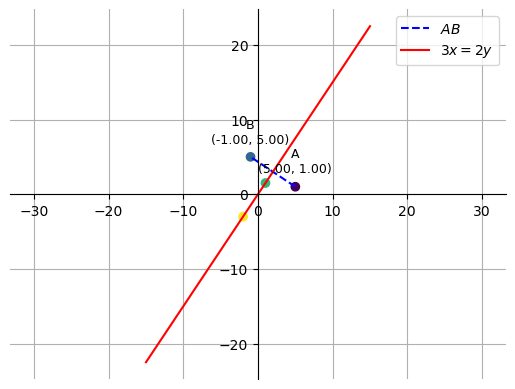
\includegraphics[width=1\textwidth]{plots/plot.png}
    \caption{Perpendicular bisector of Line AB}
    \end{figure}   
%
%The radius  of $C$ is obtained as
%\begin{align}
%r = \norm{O-P} = 2
%\end{align}
\end{frame}
%\section{Plot}
\section{C Code}
\begin{frame}[fragile]
\frametitle{C Code}
\begin{lstlisting}[language=C]
#include <stdio.h>

void print_points_to_file(const char *filename) {
    FILE *file = fopen(filename, "w");
    if (file == NULL) {
        perror("Error opening file");
        return;
    }

    // Define points A and B
    fprintf(file, "5 1\n");   // Point A
    fprintf(file, "-1 5\n");  // Point B

    // Define two points on the line 3x = 2y
    double x1 = 2, y1 = (3 * x1) / 2;
    double x2 = -2, y2 = (3 * x2) / 2;
    \end{lstlisting}
\end{frame}
\begin{frame}[fragile]
\frametitle{C Code}
\begin{lstlisting}[language=C]

    fprintf(file, "%.2lf %.2lf\n", x1, y1);  // Point on the line
    fprintf(file, "%.2lf %.2lf\n", x2, y2);  // Another point on the line

    fclose(file);
}

int main() {
    print_points_to_file("output.txt");
    return 0;
}
\end{lstlisting}
\end{frame}


\section{Python Code}
\begin{frame}[fragile]
\frametitle{Python Code for Plotting}
\begin{lstlisting}[language=Python]
import sys                                         
sys.path.insert(0, '/home/eshan/matgeo/codes/CoordGeo')      
import numpy as np
import matplotlib.pyplot as plt

#local imports
from line.funcs import *

# Function to read points from a file
def read_points_from_file(filename):
    # Load the data from the file directly into a NumPy array
    points = np.loadtxt(filename)
    return points
# Read points from file
points = read_points_from_file('output.txt')
\end{lstlisting}
\end{frame}
\begin{frame}[fragile]
\frametitle{Python Code for Plotting}
\begin{lstlisting}[language=Python]
# Flatten the array if necessary
if points.ndim == 3:
    points = points.reshape(-1, 2)

# Extracting points A, B, C, and D
A, B, C, D = points[0], points[1], points[2], points[3]

# Define a range of values for plotting infinitely
x_range = np.linspace(-15, 15, 100)  # Adjust as necessary to ensure lines extend sufficiently
# Generating all lines
x_AB = line_gen(A, B)

plt.plot(x_range,x_AB[0, :], x_AB[1, :], 'b--', label='$AB$')
# Line CD
slope_CD = (D[1] - C[1]) / (D[0] - C[0])
intercept_CD = C[1] - slope_CD * C[0]
\end{lstlisting}
\end{frame}
\begin{frame}[fragile]
\frametitle{Python Code for Plotting}
\begin{lstlisting}[language=Python]
plt.plot(x_range, slope_CD * x_range + intercept_CD, label='$3x=2y$', color='red')

# Plotting points
colors = np.arange(1, 5)  # 4 points
plt.scatter(points[:, 0], points[:, 1], c=colors, label=None)

# Annotate the vertices
def annotate_point(point, label):
    plt.annotate(f'{label}\n({point[0]:.2f}, {point[1]:.2f})',
                 point,
                 textcoords="offset points",
                 xytext=(0, 10),  # Position above the point
                 ha='center',
                 fontsize=9)              
annotate_point(A, 'A')
annotate_point(B, 'B')
\end{lstlisting}
\end{frame}
\begin{frame}[fragile]
\frametitle{Python Code for Plotting}
\begin{lstlisting}[language=Python]
# Customize the plot
ax = plt.gca()
ax.spines['top'].set_color('none')
ax.spines['left'].set_position('zero')
ax.spines['right'].set_color('none')
ax.spines['bottom'].set_position('zero')
plt.grid()  # minor
plt.axis('equal')
plt.legend(loc='best')
plt.savefig('../plots/plot.png', format='png', bbox_inches='tight')
\end{lstlisting}
\end{frame}
\end{document}
